\documentclass{article}
\usepackage[english]{babel}
\usepackage[utf8]{inputenc}
\usepackage{fancyhdr}
\usepackage{amsmath}
\usepackage{amsfonts}
\usepackage{mathrsfs}
\usepackage{mathtools}
\usepackage{indentfirst}
\usepackage{hyperref}
\usepackage{tikz,tkz-tab,amsmath}
\hypersetup{
    colorlinks=true,
    linkcolor=blue,
    filecolor=magenta,      
    urlcolor=blue,
}
\urlstyle{same}

\usepackage{scalerel,stackengine}
\stackMath
\newcommand\reallywidehat[1]{%
\savestack{\tmpbox}{\stretchto{%
  \scaleto{%
    \scalerel*[\widthof{\ensuremath{#1}}]{\kern-.6pt\bigwedge\kern-.6pt}%
    {\rule[-\textheight/2]{1ex}{\textheight}}%WIDTH-LIMITED BIG WEDGE
  }{\textheight}% 
}{0.5ex}}%
\stackon[1pt]{#1}{\tmpbox}%
}
\parskip 1ex

\usepackage{geometry}
 \geometry{
 a4paper,
 left=20mm,
 top=20mm,
 bottom=20mm,
 right=20mm
 }

\pagestyle{fancy}
\fancyhf{}
\rhead{DM}
\lhead{}
\rfoot{Page \thepage}

\makeatletter
\def\@seccntformat#1{%
  \expandafter\ifx\csname c@#1\endcsname\c@section\else
  \csname the#1\endcsname\quad
  \fi}
\makeatother

\begin{document}
% ----------------------------------------------------%
%                                                     %
%                      PARTIE 1                       %
%                                                     %
% ----------------------------------------------------%
\begin{center}
\section{Exercice 3 p.105}
\end{center}

%\subsection*{Partie A}

\textbf{1.}
\vspace{2mm}

\noindent Les primitives de la fonction $f(x)$ sont de formes : $F(x) = -e^{-kx} + K$ avec K une constante. Par exemple, une primitive particulière de cette fonction est $F(x) = -e^{-kx}$.

\vspace{2mm}
\textbf{2.}
\vspace{2mm}

\noindent L'aire du triangle $OCB$ est :

$A_{OCB} = \displaystyle\frac{1}{2}\Big(CB \times OC \Big)$

$A_{OCB} = \displaystyle\frac{1}{2} \times f(1)$

$A_{OCB} = \displaystyle\frac{1}{2} k e^{-k}$

\noindent Ensuite l'aire du domaine $\mathcal{D}$ est la soustraction de l'aire sous la courbe $\mathcal{C}_f$ (de la borne 0 à la borne 1) par l'aire $A_{OCB}$ précédemment défini du triangle $OCB$.

$A_{D} = \displaystyle\int_0^1 f(x) \: dx - A_{OCB}$

$A_{D} = \Big[-e^{-kx} \Big]_0^1 - A_{OCB}$

$A_{D} = -e^{-k} + e^0 - A_{OCB}$

$A_{D} = 1 - e^{-k} - \displaystyle\frac{1}{2} k e^{-k}$

$A_{D} = 1 - \displaystyle\frac{2 e^{-k} -  k e^{-k}}{2}$

$A_{D} = 1 - \displaystyle\frac{e^{-k}(2 + k)}{2}$

\vspace{2mm}
\textbf{3.}
\vspace{2mm}

$A_D = 2 A_{OCD}$

$\Leftrightarrow 1 - \displaystyle\frac{e^{-k}(2+k)}{2} = 2 \times \displaystyle\frac{1}{2} \times k e^{-k}$

$\Leftrightarrow 1 - \displaystyle\frac{e^{-k}(2+k)}{2} = k e^{-k}$

$\Leftrightarrow 1 - \displaystyle\frac{2e^{-k}+ke^{-k}}{2} - k e^{-k} = 0$

$\Leftrightarrow 1 - \displaystyle\frac{2e^{-k}+ke^{-k} + 2ke^{-k}}{2} = 0$

$\Leftrightarrow 1 - e^{-k} - \displaystyle\frac{3ke^{-k}}{2} = 0$

\noindent On obtient alors une fonction, que l'on nomme $g(k) = 1 - e^{-k} - \displaystyle\frac{3}{2}ke^{-k} = 0$  on cherche alors sa racine $\neq 0$. g(x) est dérivable sur $[0, +\infty[$ :

- $(1)' = 0$

- $(e^{-k})' = -e^{-k}$

- $\Big(\displaystyle\frac{3}{2}ke^{-k}\Big)' = \displaystyle\frac{3}{2}\Big(e^{-k} -ke^{-k}\Big)$  avec $u(k) = k$, $u'(k) = 1$ et $v(x) = e^{-x}$, $v'(k) = -e^{-k}$


$g(k)' = \displaystyle\frac{3}{2}\Big(e^{-k} -ke^{-k}\Big)$

$g(k)' = \displaystyle\frac{3}{2}e^{-k} - \displaystyle\frac{3}{2}ke^{-k}$

$g(k)' = e^{-k}\Big(1-\displaystyle\frac{3}{2} + \displaystyle\frac{3}{2}k \Big)$

$g(k)' = e^{-k}\Big(\displaystyle\frac{-1+3k}{2}\Big)$

\noindent On résoud $g'(k) = 0$ :

$e^{-k} \times \Big(\displaystyle\frac{-1+3k}{2} \Big) = 0$

$\Leftrightarrow \displaystyle\frac{-1+3k}{2} = 0$ (car $e^{-k}$ est strictement positif)

$\Leftrightarrow -1+3k = 0$ 

$\Leftrightarrow k = \displaystyle\frac{1}{3}$ 

$g(\frac{1}{3}) \simeq -0.07$


\vspace{2mm}

\noindent On obtient le tableau suivant :

\vspace{2mm}

{\centering
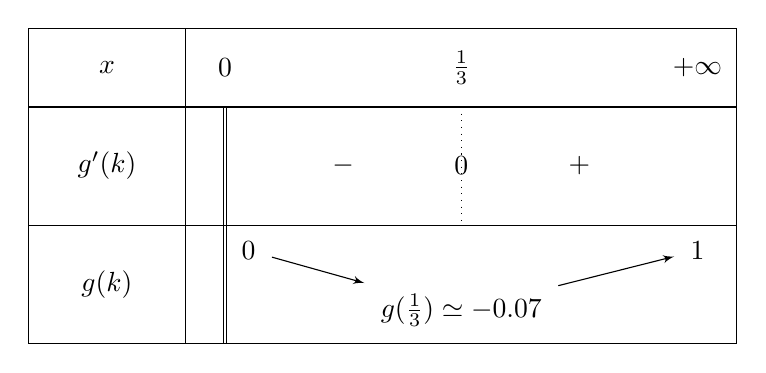
\begin{tikzpicture}
\tkzTabInit[]{$x$ /1, $g'(k)$ /1.5,  $g(k)$ /1.5}{$0$, $\frac{1}{3}$, $+\infty$}%
\tkzTabLine{d,-,z,+}
\tkzTabVar{D+/$0$, -/$g(\frac{1}{3}) \simeq -0.07$, +/$1$}
\end{tikzpicture}
\par}

\vspace{2mm}

\noindent D'après le tableau de variation, la fonction $g(k)$ est continue et strictement croissante sur $]0; +\infty[$; l'image de $]0; +\infty[$ par $g$ est $]0, 1]$ qui contient 0 car l'extremum entre la borne inférieur et supérieur est $g(\frac{1}{3}) = \displaystyle\frac{1}{3}$. D'après le corollaire du théorème des valeurs intermédiaires l'équation $g(x) = 0$ admet une seule solution sur $]0, +\infty[$. Donc on peut dire qu'il existe une unique valeur du réel k strictement positive telle que l'aire du domaine $\mathcal{D}$ vaut le double de celle du triangle $\mathcal{OCB}$

% ----------------------------------------------------%
%                                                     %
%                      PARTIE 2                       %
%                                                     %
% ----------------------------------------------------%
\vspace{4mm}
\begin{center}
\section{Exercice 1 p.18}
\end{center}

\subsection*{Partie A}

\textbf{A.1.a}

\[
    \left.\begin{matrix*}[r]
       \displaystyle\lim_{x\rightarrow+\infty} \displaystyle\frac{7}{2} = \displaystyle\frac{7}{2}\\
       \\
       \\
       \left.\begin{matrix*}[r]
            \left.\begin{matrix*}
                \displaystyle\lim_{x\rightarrow+\infty} e^{x} = +\infty\\
               \\
               \displaystyle\lim_{x\rightarrow+\infty} e^{-x} = 0\\
            \end{matrix*}\medspace\right\}
            \left.\begin{matrix*}
                \space\text{par somme :}
                \vspace{2mm}\\
                \displaystyle\lim_{x\rightarrow+\infty} \displaystyle e^x+e^{-x} = +\infty
            \end{matrix*}\right.    
           \\
           \\
           \displaystyle\lim_{x\rightarrow\infty} -\displaystyle\frac{1}{2} = -\displaystyle\frac{1}{2}\\
        \end{matrix*}\medspace\right\}
        \left.\begin{matrix*}
            \space\text{par produit :}\vspace{2mm}\\
            \displaystyle\lim_{x\rightarrow+\infty} -\displaystyle\frac{1}{2}\Big(e^x + e^{-x}\Big) = -\infty
        \end{matrix*}\right.
    \end{matrix*}\medspace\right\}
    \left.\begin{matrix*}
        \space\text{par somme :}\vspace{2mm}\\
        \displaystyle\lim_{x\rightarrow+\infty}  
        f(x) = -\infty
    \end{matrix*}\right.
\] 


\vspace{2mm}

\textbf{A.1.b}

\vspace{2mm}

\noindent $f(x)$ est dérivable sur $[0, \infty[$ est de forme $u(x) \times v(x)$ avec :

- $u(x) = -\displaystyle\frac{1}{2}$
- $u'(x) = 0$
- $v(x) = (e^{x}+e^{-x})$
- $v'(x) = e^x-e^{-x}$

\noindent donc :

$f'(x) = u'(x) \times v(x) + u'(x) \times u(x) = 0 \times (e^x+e^{-x}) + (e^x-e^{-x}) \times -\displaystyle\frac{1}{2} = -\displaystyle\frac{1}{2}(e^x-e^{-x})$

\vspace{2mm}

\noindent Signe de $e^x-e^{-x}$ :

$e^x - e^{-x} > 0 \Leftrightarrow e^x > e^{-x} \Leftrightarrow ln(e^x) > ln(e^{-x})$

$\Leftrightarrow x > -x \Leftrightarrow 2x > 0 \Leftrightarrow x > 0$

\vspace{3mm}

{\centering
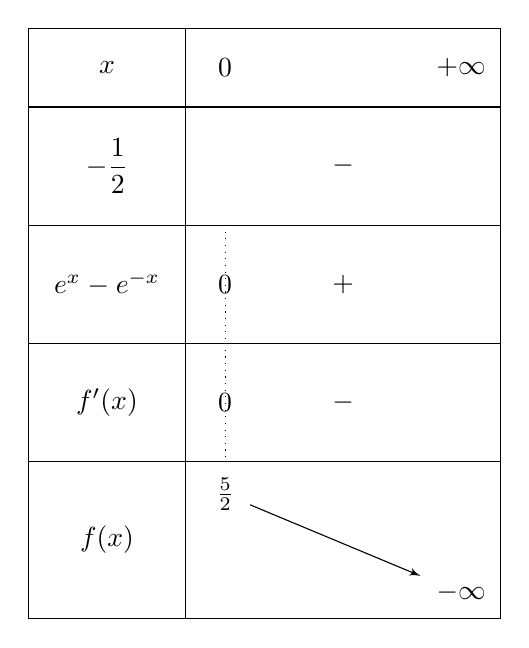
\begin{tikzpicture}
\tkzTabInit[]{$x$ /1, $-\displaystyle\frac{1}{2}$ /1.5,  $e^x-e^{-x}$ /1.5, $f'(x)$ /1.5, $f(x)$ /2}{$0$, $+\infty$}%
\tkzTabLine{,-,}
\tkzTabLine{z,+,}
\tkzTabLine{z,-,}
\tkzTabVar{+/$\frac{5}{2}$, -/$-\infty$}
\end{tikzpicture}
\par}


\vspace{2mm}

\textbf{A.1.c}

\vspace{2mm}

\noindent $f(0) = \displaystyle\frac{7}{2} - \displaystyle\frac{1}{2}\Big(e^0 + e^{0}\Big) = \displaystyle\frac{7}{2} - \displaystyle\frac{1}{2}\times 2 = \displaystyle\frac{7}{2} - 1 = \displaystyle\frac{5}{2}$

\vspace{2mm}

\noindent D'après le tableau de variation, la fonction f est continue et strictement décroissante sur $[0; +\infty[$; l'image de $[0; +\infty[$ est $[2.5; -\infty[$ qui contient 0. D'après le corollaire du théorème des valeurs intermédiaires l'équation $f(x) = 0$ admet une seule solution $\alpha$ sur $[0; +\infty[$.

\vspace{2mm}

\subsection*{Partie B}

\textbf{B.1}

\noindent La hauteur h d'un arceau correspond à la valeur de $f(0)$ selon le schéma. On a déjà calculé la valeur de $f(0)$ dans la question A.1.c. Donc $h = f(0) = \displaystyle\frac{5}{2} = 2.5$

\textbf{B.2.a}

\vspace{2mm}

$1+(f'(x))^2$

$= 1 + \Bigg(\displaystyle\frac{1}{2}\Big(e^{-x}-e^{x}\Big)\Bigg)^2$

$= 1 + \displaystyle\frac{1}{4}\Big(e^{-x}-e^{x}\Big)^2$

$= 1 + \displaystyle\frac{1}{4}\Big((e^{-x})^2 - 2e^{-x} \times e^{x} + (e^{x})^2 \Big)$

$= 1 + \displaystyle\frac{1}{4}\Big( e^{-2x} - 2e^{-x + x} + e^{2x} \Big)$

$= 1 + \displaystyle\frac{1}{4}\Big( e^{-2x} - 2 + e^{2x} \Big)$

$= \displaystyle\frac{4 + e^{-2x} - 2 + e^{2x}}{4}$

$= \displaystyle\frac{1}{4}\Big((e^{-x})^2 + 2 + (e^{x})^2\Big)$

$= \displaystyle\frac{1}{4}\Big((e^{-x})^2 + 2 \times e^{-x} \times e^x + (e^{x})^2\Big)$

$= \displaystyle\frac{1}{4}\Big(e^x + e^{-x}\Big)^2$

\vspace{1mm}
\noindent Donc on a bien :
\vspace{1mm}

$1 + (f'(x))^2 = \displaystyle\frac{1}{4}\Big(e^x+e^{-x}\Big)^2$

\vspace{2mm}
\textbf{B.2.b}
\vspace{2mm}

$I = \displaystyle\int_0^{\alpha}\sqrt{1+(f'(x))^2} dx$

\noindent On utilise le résultat de la question 2.b:

$I = \displaystyle\int_0^{\alpha}\sqrt{\displaystyle\frac{1}{4}\Big(e^x + e^{-x}\Big)^2} dx$

$I = \displaystyle\int_0^{\alpha}\displaystyle\frac{1}{2}\Big(e^x + e^{-x}\Big) dx$

$I = \displaystyle\int_0^{\alpha}\displaystyle\frac{1}{2}\Big(e^x + e^{-x}\Big) dx$

$I = \displaystyle\frac{1}{2} \displaystyle\int_0^{\alpha}e^x + e^{-x} dx$

$I = \displaystyle\frac{1}{2} \Big[e^x + \displaystyle\frac{1}{-1} e^{-x}\Big]_0^\alpha$

$I = \displaystyle\frac{1}{2} \Big[e^x - e^{-x}\Big]_0^\alpha$

$I = \displaystyle\frac{1}{2} \big(e^{\alpha} - e^{-\alpha} + e^0- e^0 \big)$

$I = \displaystyle\frac{1}{2} \big(e^{\alpha} - e^{-\alpha} \big)$

\vspace{2mm}

\noindent La longueur d'un arceau constitue le double de I. 
Vu que la fonction $f(x)$ est paire alors la longueur de la courbe $C$ sur $[-\alpha, 0]$ est égale à celle sur $[0, \alpha]$. 
Donc la longueur d'un arceau est égale à $2I$, soit $e^{\alpha}-e^{-\alpha}$.

\vspace{2mm}
\textbf{C.1.a}
\vspace{2mm}

\noindent Comme fonction $f(x)$ est paire alors l'intégrale $\int^{\alpha}_0 f(x) \space dx$ représente la moitié de l'aire d'une façade complète. Donc l'expression $4 \int^{\alpha}_0 f(x) \space dx$ représente les deux aires complètes des deux façades. On soustrait 2 à cette expression pour enlever l'aire de l'ouverture d'aire $1 \times 2 = 2 \space m^2$.

\vspace{2mm}
\textbf{C.2.b}
\vspace{2mm}

\noindent On note $\mathcal{A}_F$ l'aire des deux façades.

$\mathcal{A}_{F} = 4\displaystyle\int_0^{\alpha} f(x) \: dx - 2$

$\mathcal{A}_{F} = 4\displaystyle\int_0^{\alpha} \displaystyle\frac{7}{2} - \displaystyle\frac{1}{2} \Big(e^x + e^{-x}\Big) \: dx - 2$

$\mathcal{A}_{F} = 4 \Bigg[ \displaystyle\frac{7}{2}x - \displaystyle\frac{1}{2}(e^x - e^{-x}) \Bigg]^{\alpha}_0 - 2$

$\mathcal{A}_{F} = 4 \Bigg( \displaystyle\frac{7}{2}\alpha - \displaystyle\frac{1}{2}(e^{\alpha} - e^{-\alpha}) - \displaystyle\frac{7}{2} \times 0 - \displaystyle\frac{1}{2}(e^0 - e^{0}) \Bigg) - 2$

$\mathcal{A}_{F} = 4 \Bigg( \displaystyle\frac{7}{2}\alpha - \displaystyle\frac{1}{2}(e^{\alpha} - e^{-\alpha}) \Bigg) - 2$

$\mathcal{A}_{F} = 14\alpha - 2(e^{\alpha} - e^{-\alpha}) - 2$

\vspace{2mm}

\noindent D'après l'énoncé, l'aire du dessus de la serre correspond à un rectangle de $1,50 \times 3 = 4,5 m$ par $I$ m donc l'aire du dessus noté $\mathcal{A}_F$ est :

\vspace{2mm}

$\mathcal{A}_{D} = 1,50 \times 3 \times I = 4,5I = 4,5(e^{\alpha} - e^{-\alpha})$

$\mathcal{A}_{T} = \mathcal{A}_{F} + \mathcal{A}_{D} $

$\mathcal{A}_{T} = 14\alpha - 2(e^{\alpha} - e^{-\alpha}) - 2 + 4,5(e^{\alpha} - e^{-\alpha})$

\vspace{2mm}

\noindent Avec $\alpha = 1,92m$ on calcule l'aire totale  $\mathcal{A}_T$ :

\vspace{2mm}

$\mathcal{A}_{T} = 14 \times 1,92 - 2(e^{1,92} - e^{-1,92}) - 2 + 4,5(e^{1,92} - e^{-1,92}) \simeq 42 \: m^2$

\end{document}
